
\documentclass[oneside,letterpaper,12pt]{book}
\usepackage{Rd}
\usepackage{/usr/lib64/R/share/texmf/Sweave}
\usepackage{bibentry}
\usepackage{upquote}
\usepackage{graphicx}
\usepackage{natbib}
\usepackage[reqno]{amsmath}
\usepackage{amssymb}
\usepackage{amsfonts}
\usepackage{amsmath}
\usepackage{verbatim}
\usepackage{epsf}
\usepackage{url}
\usepackage{html}
\usepackage{dcolumn}
\usepackage{multirow}
\usepackage{fullpage}
\usepackage{lscape}
\usepackage[all]{xy}
% \usepackage[pdftex, bookmarksopen=true,bookmarksnumbered=true,
%   linkcolor=webred]{hyperref}
\bibpunct{(}{)}{;}{a}{}{,}
\newcolumntype{.}{D{.}{.}{-1}}
\newcolumntype{d}[1]{D{.}{.}{#1}}
\htmladdtonavigation{
  \htmladdnormallink{%
    \htmladdimg{http://gking.harvard.edu/pics/home.gif}}
  {http://gking.harvard.edu/}}
\newcommand{\MatchIt}{{\sc MatchIt}}
\newcommand{\hlink}{\htmladdnormallink}
\newcommand{\Sref}[1]{Section~\ref{#1}}
\newcommand{\fullrvers}{2.5.1}
\newcommand{\rvers}{2.5}
\newcommand{\rwvers}{R-2.5.1}
%\renewcommand{\bibentry}{\citealt}

\bodytext{ BACKGROUND="http://gking.harvard.edu/pics/temple.jpg"}
\setcounter{tocdepth}{2}

%\VignetteIndexEntry{ARIMA Models for Time Series Data}
%\VignetteDepends{Zelig}
%\VignetteKeyWords{model,time series}
%\VignettePackage{Zelig}
\usepackage{Sweave}
\begin{document}
\nobibliography*
\nobibliography*

\section{{\tt ARIMA}: ARIMA Models for Time Series Data}
\label{ARIMA} 

Use auto-regressive, integrated, moving-average (ARIMA) models for
time series data.  A time series is a set of observations ordered
according to the time they were observed.  Because the value observed
at time $t$ may depend on values observed at previous time points,
time series data may violate independence assumptions.  An ARIMA($p$,
$d$, $q$) model can account for temporal dependence in several ways.
First, the time series is differenced to render it stationary, by
taking $d$ differences.  Second, the time dependence of the stationary
process is modeled by including $p$ auto-regressive and $q$
moving-average terms, in addition to any time-varying covariates.  For
a cyclical time series, these steps can be repeated according to the
period of the cycle, whether quarterly or monthly or another time
interval.  ARIMA models are extremely flexible for continuous data.
Common formulations include, ARIMA(0, 0, 0) for least squares
regression (see \Sref{ls}), ARIMA(1, 0, 0), for an AR1 model, and
ARIMA(0, 0, 1) for an MA1 model.  For a more comprehensive review of
ARIMA models, see \cite{Enders04}.

\subsubsection*{Syntax}
\begin{verbatim}
> z.out <- zelig(Diff(Y, d, ds=NULL, per=NULL) ~ lag.y(p, ps=NULL) 
                 + lag.eps(q, qs=NULL) + X1 + X2, 
                 model="arima", data=mydata, ...)
> x.out <- setx(z.out, X1 = list(time, value), cond = FALSE) 
> s.out <- sim(z.out, x=x.out, x1=NULL)
\end{verbatim}

\subsubsection*{Inputs}
In addition to independent variables, {\tt zelig()} accepts the
following arguments to specify the {\tt ARIMA} model:
\begin{itemize}
\item {\tt Diff(Y, d, ds, per)} for a dependent variable Y sets the
number of non-seasonal differences ({\tt d}), the number of seasonal differences ({\tt
ds}), and the period of the season ({\tt per}).
\item {\tt lag.y(p, ps)} sets the number of lagged observations of the
dependent variable for non-seasonal ({\tt p}) and seasonal ({\tt ps})
components.
\item {\tt lag.eps(q, qs)} sets the number of lagged innovations, or
differences between the observed value of the time series and the
expected value of the time series for non-seasonal ({\tt q}) and
seasonal ({\tt qs}) components.  
\end{itemize}
In addition the user can control the estimation of the time
series with the following terms: 
\begin{itemize}
\item $\hdots$: Additional inputs.  See {\tt help(arima)} in the stats
library for further information.
\end{itemize}
  
\subsubsection*{Stationarity}
A stationary time series has finite variance, correlations between
observations that are not time-dependent, and a constant expected
value for all components of the time series \citep[p.\ 12]{BroDav91}.
Users should ensure that the time series being analyzed is stationary
before specifying a model.  The following commands provide diagnostics
to determine if a time series {\tt Y} is stationary.
\begin{itemize}
\item {\tt pp.test(Y)}: Tests the null hypothesis that the time series
  is non-stationary.  
\item {\tt kpss.test(Y)}: Tests the null hypothesis that the time
  series model is stationary.
\end{itemize}  
The following commands provide graphical means of diagnosing whether a
given time series is stationary.  
\begin{itemize}
\item {\tt ts.plot(Y)}: Plots the observed time series.  
\item {\tt acf(Y)}: Provides the sample auto-correlation function
(correlogram) for the time series.
\item {\tt pacf(Y)}: Provides the sample partial auto-correlation
  function (PACF) for the time series.  \\
\end{itemize}
These latter two plots are also useful in determining the $p$
autoregressive terms and the $q$ lagged error terms.  See
\cite{Enders04} for a complete description of how to utilize ACF and
PACF plots to determine the order of an ARIMA model.

\subsubsection*{Examples}

\begin{enumerate}

\item No covariates\newline

Estimate the ARIMA model, and summarize the results.
\begin{Schunk}
\begin{Sinput}
> data(approval)
\end{Sinput}
\end{Schunk}
\begin{Schunk}
\begin{Sinput}
> z.out1 <- zelig(Diff(approve, 1) ~ lag.eps(2) + lag.y(2), data = approval, 
+     model = "arima")
> summary(z.out1)
\end{Sinput}
\end{Schunk}
Set the number of time periods (ahead) for the prediction to run.
for which you would like the prediction to run:
\begin{Schunk}
\begin{Sinput}
> x.out1 <- setx(z.out1, pred.ahead = 10)
\end{Sinput}
\end{Schunk}
Simulate the predicted quantities of interest:
\begin{Schunk}
\begin{Sinput}
> s.out1 <- sim(z.out1, x = x.out1)
\end{Sinput}
\end{Schunk}
Summarize and plot the results:
\begin{Schunk}
\begin{Sinput}
> summary(s.out1)
\end{Sinput}
\end{Schunk}
\begin{center}
\begin{Schunk}
\begin{Sinput}
> plot(s.out1, lty.set = 2)
\end{Sinput}
\end{Schunk}
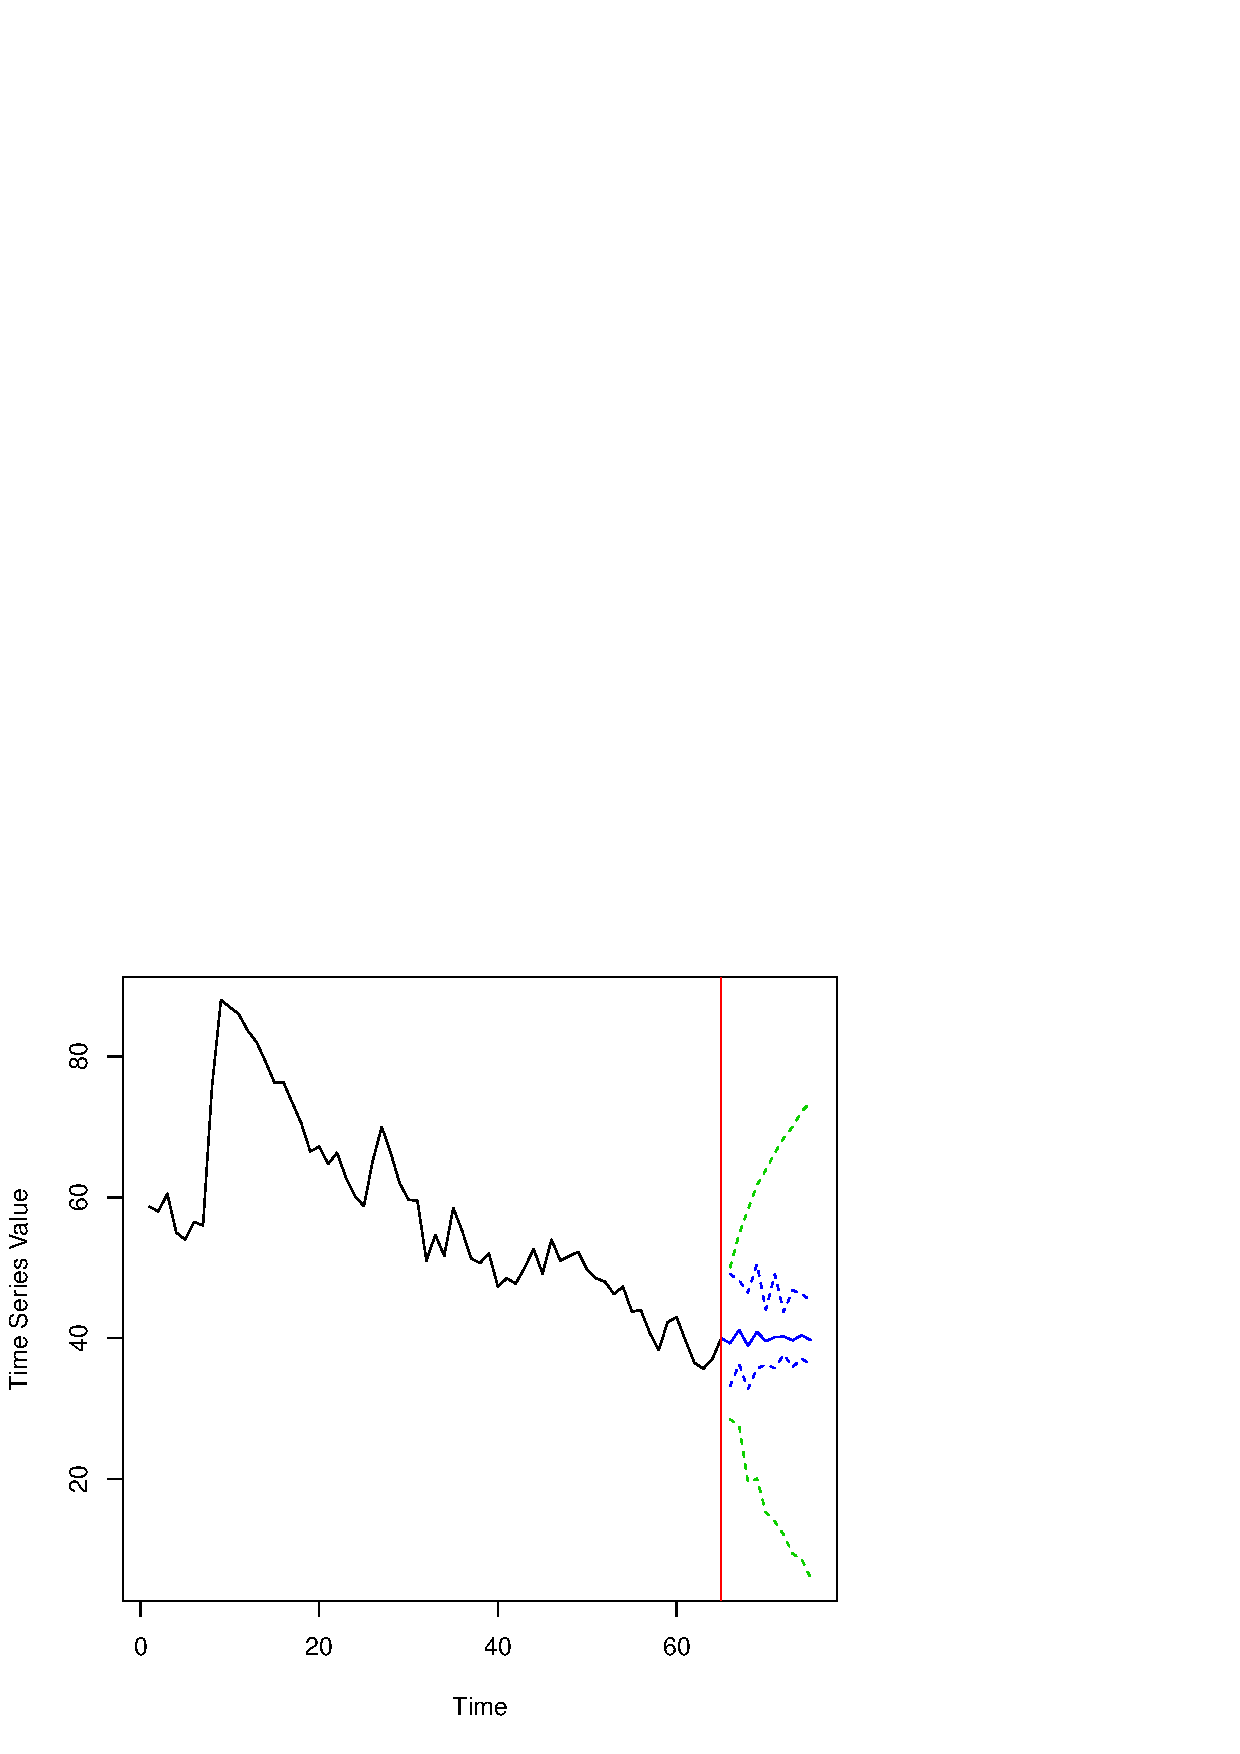
\includegraphics{vigpics/arima-Example1Plot}
\end{center}

\item Calculating a treatment effect\newline

Estimate an ARIMA model with exogenous regressors, in addition to
lagged errors and lagged values of the dependent variable.

\begin{Schunk}
\begin{Sinput}
> z.out2 <- zelig(Diff(approve, 1) ~ iraq.war + sept.oct.2001 + 
+     avg.price + lag.eps(1) + lag.y(2), data = approval, model = "arima")
\end{Sinput}
\end{Schunk}
To calculate a treatment effect, provide one counterfactual value for
one time period for one of the exogenous regressors (this is the
counterfactual treatment). 
\begin{Schunk}
\begin{Sinput}
> x.out2 <- setx(z.out2, sept.oct.2001 = list(time = 45, value = 0), 
+     cond = T)
\end{Sinput}
\end{Schunk}
Simulate the quantities of interes
\begin{Schunk}
\begin{Sinput}
> s.out2 <- sim(z.out2, x = x.out2)
\end{Sinput}
\end{Schunk}
Summarizing and plotting the quantities of interest.
\begin{Schunk}
\begin{Sinput}
> summary(s.out2)
\end{Sinput}
\end{Schunk}
%the plot does not work 
\begin{center}
\begin{Schunk}
\begin{Sinput}
> plot(s.out2)
\end{Sinput}
\end{Schunk}
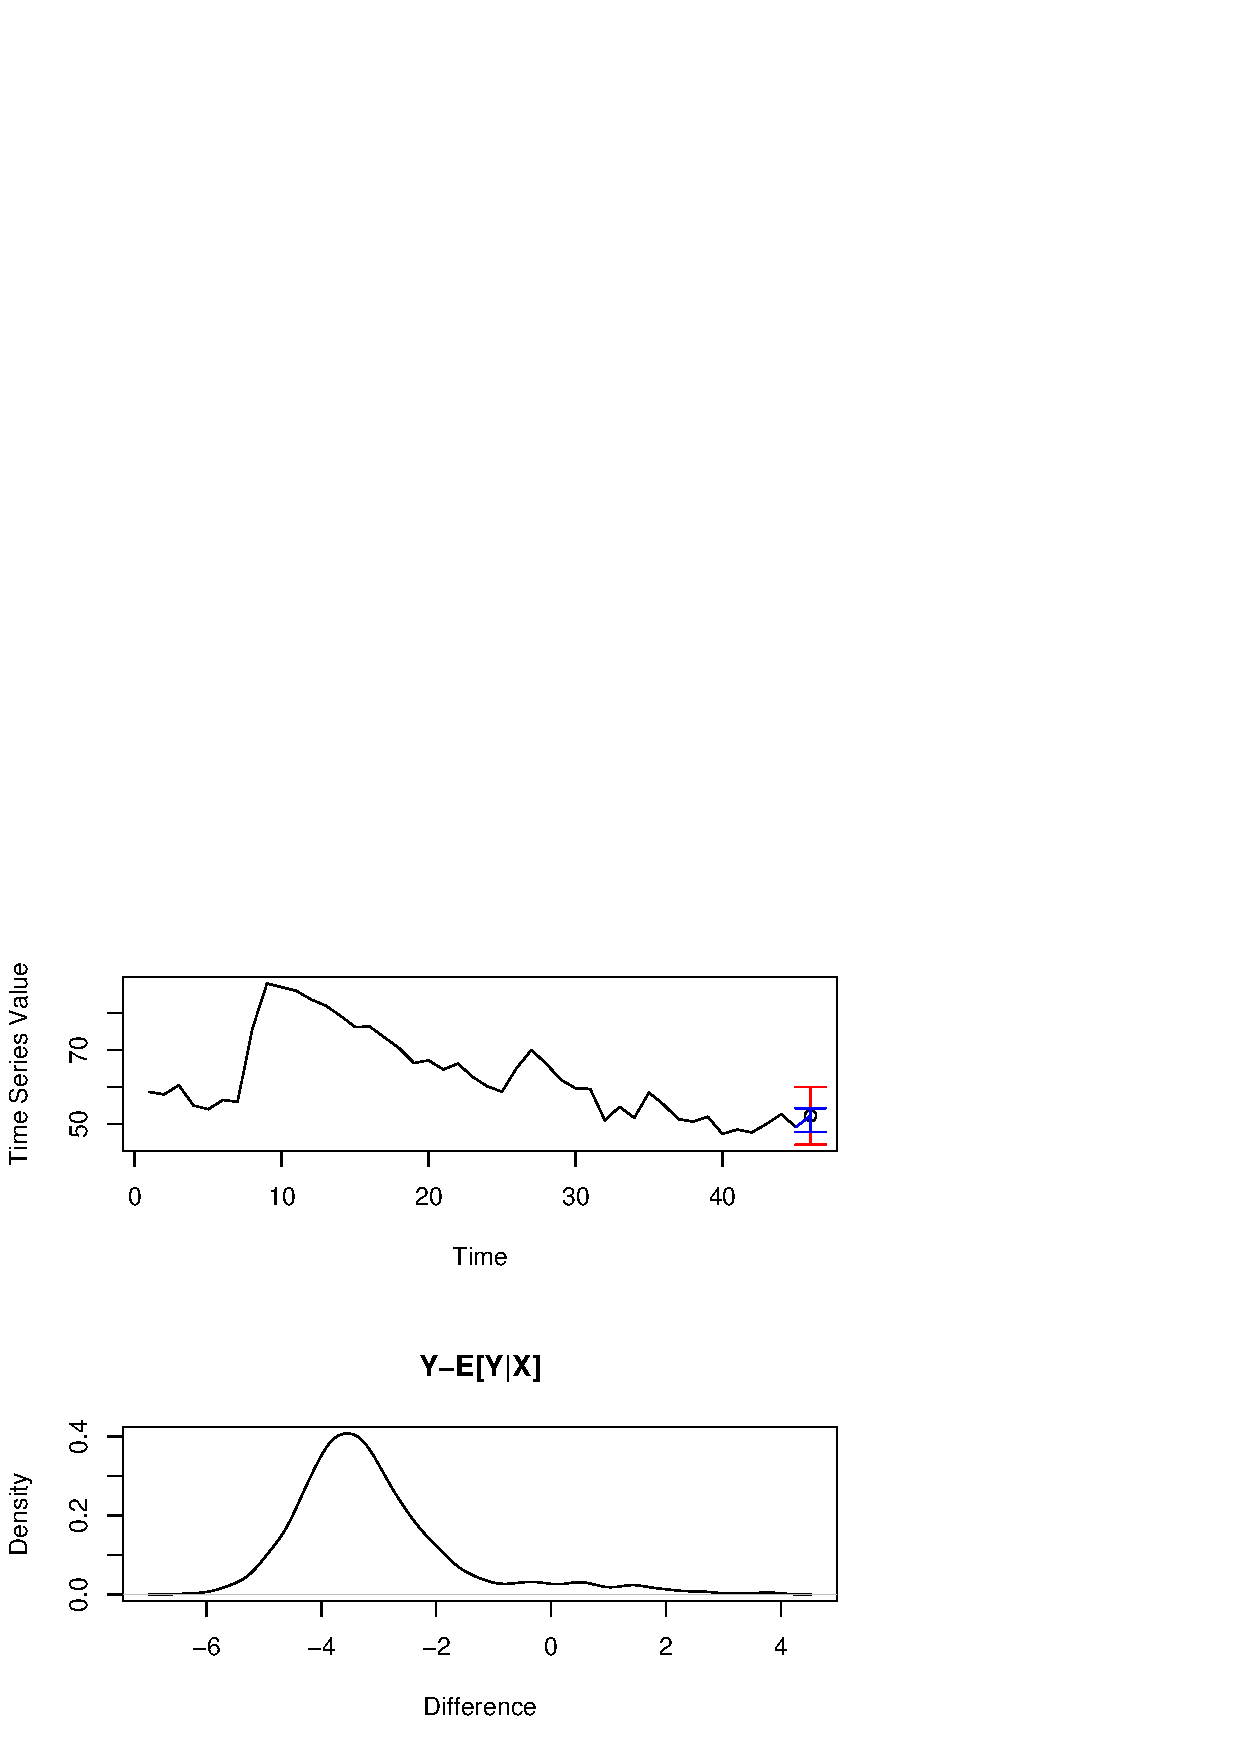
\includegraphics{vigpics/arima-Example2Plot}
\end{center}

\item Calculating first differences\newline

Continuing the example from above, calculate first differences by
selecting several counterfactual values for one of the exogenous
regressors. 
\begin{Schunk}
\begin{Sinput}
> x.out3 <- setx(z.out2, sept.oct.2001 = list(time = 45:50, value = 0))
> x1.out3 <- setx(z.out2, sept.oct.2001 = list(time = 45:50, value = 1))
\end{Sinput}
\end{Schunk}
Simulating the quantities of interest
\begin{Schunk}
\begin{Sinput}
> s.out3 <- sim(z.out2, x = x.out3, x1 = x1.out3)
\end{Sinput}
\end{Schunk}
Summarizing and plotting the quantities of interest. Choosing {\tt
pred.se = TRUE} only displays the uncertainty resulting from parameter
estimation.  
\begin{Schunk}
\begin{Sinput}
> summary(s.out3)
\end{Sinput}
\end{Schunk}
%the plot does not work
\begin{center}
\begin{Schunk}
\begin{Sinput}
> plot(s.out3, pred.se = TRUE)
\end{Sinput}
\end{Schunk}
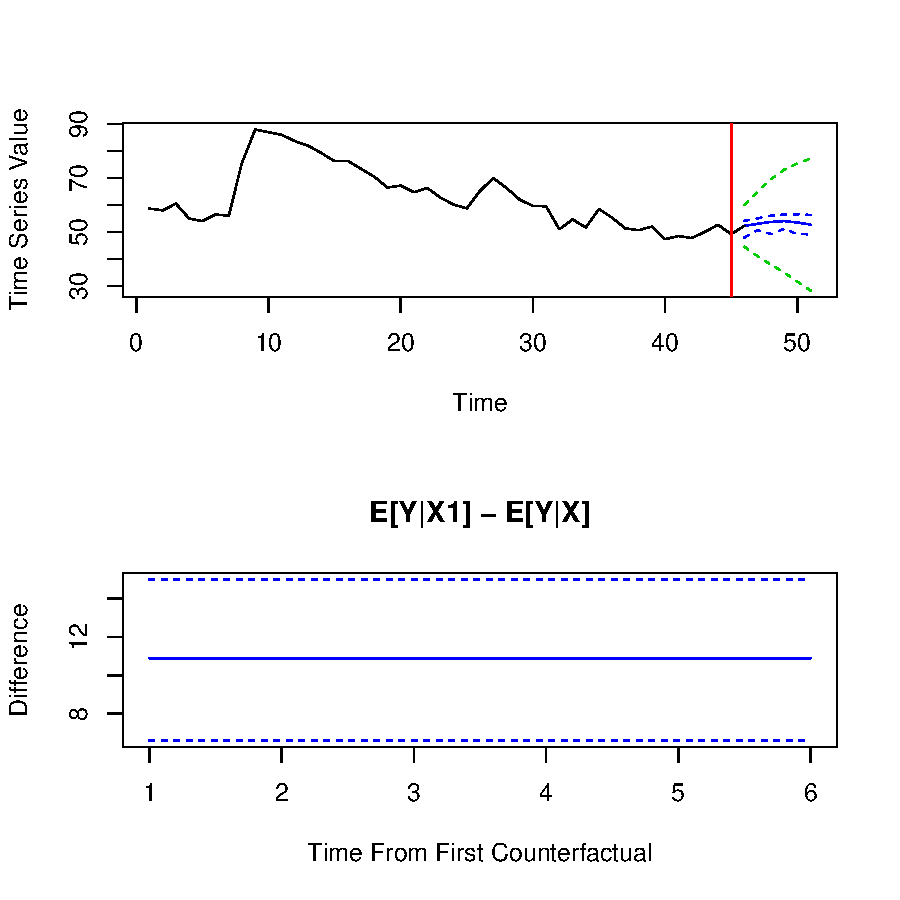
\includegraphics{vigpics/arima-Example3Plot}
\end{center} 
\end{enumerate}

\subsubsection*{Model}
Suppose we observe a time series $Y$, with observations $Y_i$ where
$i$ denotes the time at which the observation was recorded.  The first
step in the ARIMA procedure is to ensure that this series is
stationary.  If initial diagnostics indicate non-stationarity, then we
take additional differences until the diagnostics indicate
stationarity.  Formally, define the difference operator, $\nabla^
{d}$, as follows.  When $d = 1$, $\nabla^{1} Y = Y_i - Y_{i-1}$, for
all observations in the series.  When $d=2$, $\nabla^2 Y = (Y_{i} -
Y_{i-1}) - (Y_{i-1} - Y_{i-2})$.  This is analogous to a polynomial
expansion, $Y_{i} - 2Y_{i-1} + Y_{i-2}$.  Higher orders of
differencing ($d > 2$) following the same function.  Let $Y^*$
represent the stationary time series derived from the initial time
series by differencing $Y$ $d$ times.  In the second step, lagged
values of $Y^{*}$ and errors $\mu - Y^*_i$ are used to model the time
series.  ARIMA utilizes a state space representation of the ARIMA
model to assemble the likelihood and then utilizes maximum likelihood
to estimate the parameters of the model.  See \cite{BroDav91} Chapter
12 for further details.
\begin{itemize}
\item A stationary time series $Y_i^*$ that has been differenced $d$
times has \textit{stochastic component}:
\begin{equation*} 
Y_i^* \sim \text{Normal} (\mu_i, \sigma^2),
\end{equation*}
where $\mu_i$ and $\sigma^2$ are the mean and variance of the Normal
distribution, respectively.  
\item The \textit{systematic component}, $\mu_i$ is modeled as
\begin{equation*}
\mu_i = x_i \beta + \alpha_1 Y_{i-1}^* + \hdots + \alpha_p Y_{i-p}^*
+ \gamma_1\epsilon_{i-1} + \hdots + \gamma_q \epsilon_{i-q}
\end{equation*}
where $x_i$ are the explanatory variables with associated parameter
vector $\beta$; $Y^*$ the lag-$p$ observations from the stationary time
series with associated parameter vector $\alpha$; and $\epsilon_i$ the
lagged errors or innovations of order $q$, with associated parameter vector
$\gamma$.   
\end{itemize}

\subsubsection*{Quantities of Interest}
\begin{itemize}
\item The expected value ({\tt qi\$ev}) is the mean of simulations
  from the stochastic component, 
\begin{equation*}
\text{E(}Y_\text{i}) = \mu_i = x_i \beta + \alpha_1 Y_{i-1}^* + \hdots + \alpha_p Y_{i-p}^*
+ \gamma_1\epsilon_{i-1} + \hdots + \gamma_q \epsilon_{i-q}
\end{equation*}
given draws of $\beta$, $\alpha$, and $\gamma$ from their estimated
distribution.
\item The first difference ({\tt qi\$fd}) is: 
\begin{equation*}
\text{FD}_i= E(Y | x_{1i}) - E(Y|x_{i})  
\end{equation*}
\item The treatment effect ({\tt qi\$t.eff}), obtained with {\tt
setx(\dots, cond = TRUE)}, represents the difference
between the observed time series and the expected value of a time
series with counterfactual values of the external regressors.  Formally,
\begin{equation*}
\text{t.eff}_\text{i} = Y_i - E[Y_i | x_{i}] 
\end{equation*}
Zelig will not estimate both first differences and treatment effects.
\end{itemize}

\subsubsection*{Output Values}
The output of each Zelig command contains useful information which the
user may view.  For example, if the user runs {\tt z.out <-
zelig(Diff(Y,1) + lag.y(1) + lag.eps(1) + X1, model = "arima", data)}
then the user may examine the available information in {\tt z.out} by
using {\tt names(z.out)}, see the coefficients by using {\tt
z.out\$coef} and a default summary of information through {\tt
summary(z.out)}.  {\tt tsdiag(z.out)} returns a plot of the residuals,
the ACF of the residuals, and a plot displaying the $p$-values for the
Ljung-Box statistic.  Other elements, available through the \$
operator are listed below.
\begin{itemize}
\item From the {\tt zelig()} output object {\tt z.out}, you may
  extract: 
\begin{itemize}
\item {\tt coef}: parameter estimates for the explanatory variables,
lagged observations of the time series, and lagged innovations.  
\item {\tt sigma2}: maximum likelihood estimate of the variance of
the stationary time series.
\item {\tt var.coef}: variance-covariance matrix for the parameters.
\item {\tt loglik}: maximized log-likelihood.
\item {\tt aic}: Akaike Information Criterion (AIC) for the maximized
  log-likelihood.
\item {\tt residuals}: Residuals from the fitted model.
\item {\tt arma}: A vector with seven elements corresponding to the AR
and MA, the seasonal AR and MA, the period of the seasonal component,
and the number of non-seasonal and seasonal differences of the
dependent variable.
\item {\tt data}: the name of the input data frame.   
\end{itemize}
\item From the {\tt sim()} output object {\tt s.out} you may extract
  quantities of interest arranged as matrices, with the rows
  indicating the number of the simulations, and the columns
  representing the simulated value of the dependent variable for the
  counterfactual value at that time period.  {\tt summary(s.out)}
  provides a summary of the simulated values, while {\tt plot(s.out)}
  provides a graphical representation of the simulations.  Available
  quantities are:
\begin{itemize}
\item {\tt qi\$ev}: the simulated expected probabilities for the
  specified values of {\tt x}.  
\item {\tt qi\$fd} : the simulated first difference for the values
  that are specified in {\tt x} and {\tt x1}.
\item{ \tt qi\$t.eff}: the simulated treatment effect, difference
between the observed {\tt y} and the expected values given the
counterfactual values specified in {\tt x}.     
\end{itemize}  
\end{itemize}


\subsection* {How to Cite} 

To cite the \emph{ arima } Zelig model:
 \begin{verse}
 Justin Grimmer. 2007. "arima: Arima models for Time Series Data" in Kosuke Imai, Gary King, and Olivia Lau, "Zelig: Everyone's Statistical Software,"\url{http://gking.harvard.edu/zelig} 
\end{verse}
To cite Zelig as a whole, please reference these two sources:
\begin{verse}
  Kosuke Imai, Gary King, and Olivia Lau. 2007. ``Zelig: Everyone's
  Statistical Software,'' \url{http://GKing.harvard.edu/zelig}.
\end{verse}
\begin{verse}
Imai, Kosuke, Gary King, and Olivia Lau. (2008). ``Toward A Common Framework for Statistical Analysis and Development.'' Journal of Computational and Graphical Statistics, Vol. 17, No. 4 (December), pp. 892-913. 
\end{verse}


\subsection* {See also}

The ARIMA function is part of the stats package \citep{VenRip02}
For an accessible introduction to identifying the order of an ARIMA
model consult \cite{Enders04}
In addition, advanced users may wish to become more familiar with the state-space representation of an ARIMA process \citep{BroDav91}
Additional options for ARIMA models may be found using {\tt
help(arima)}.  

%\end{itemize}
\bibliographystyle{asa}
\bibliography{gk,gkpubs}

  
\bibliographystyle{asa}
\bibliography{gk,gkpubs}
\end{document}
